\documentclass[a4paper,11pt]{report}

\usepackage[utf8]{inputenc}
\usepackage[T1]{fontenc}
\usepackage[spanish,es-tabla,es-noquoting]{babel}
\usepackage{geometry}
\usepackage{array}
\usepackage{booktabs}
\usepackage{listings}
\usepackage{tikz}
\usepackage{hyperref}
\usetikzlibrary{positioning,arrows.meta}

\geometry{margin=2.8cm}
\setlength{\emergencystretch}{2em}
\setlength{\intextsep}{22pt plus 4pt minus 4pt}
\setlength{\floatsep}{22pt plus 4pt minus 4pt}
\setlength{\textfloatsep}{22pt plus 4pt minus 4pt}

% Bloque de coste: "Coste:" en negrita y separado del codigo y del texto siguiente
\newcommand{\coste}[1]{\par\bigskip\noindent\textbf{Coste:} #1\par\bigskip}

\renewcommand{\chaptername}{Capítulo}
\renewcommand{\contentsname}{Índice}
\renewcommand{\listtablename}{Índice de tablas}
\renewcommand{\lstlistingname}{Listado}

\lstset{ % Esto nos permite escribir normal sin tener que escapar acentos
    basicstyle=\small\ttfamily,
    columns=fullflexible,
    keepspaces=true,
    breaklines=true,
    frame=single,
    numbers=left,
    numberstyle=\tiny,
    showstringspaces=false,
    tabsize=4,
    literate=
        {á}{{\'a}}1 {é}{{\'e}}1 {í}{{\'i}}1 {ó}{{\'o}}1 {ú}{{\'u}}1
        {ñ}{{\~n}}1
}
% Title Page

\title{Práctica 2\\Listas doblemente enlazadas circulares}
\author{Samuel Carrasco Santurde\\Alexander Tomás Echevarria Pizarro\\Erasmo Seebold Guadilla}
\date{}


\begin{document}
\maketitle
\tableofcontents
\listoftables

\chapter{Introducción}

En esta práctica hemos implementado una estructura basada en listas enlazadas, concretamente listas doblemente enlazadas circulares.

A partir de la clase común \texttt{DoubleLinkedList} hemos creado una variante sin orden \texttt{UnorderedDoubleLinkedList} y otra con orden \texttt{OrderedDoubleLinkedList}.

El nodo \texttt{Node<T>} guarda referencias a anterior y a siguiente, lo que nos permite recorrer la lista de manera bidireccional conectando el primero con el último.

La lista ordenada tiene la restricción de que ha de implementar elementos que implementen \texttt{Comparable<T>}, mientras que la no ordenada tiene más libertad en cuanto a los elementos que almacena.

Se han realizado pruebas tanto con enteros y con objetos \texttt{Persona} para finalmente implementarlo en la práctica 1 de Actores y películas.


\section{Objetivos y alcance}

Los objetivos principales son:
\begin{itemize}
    \item Especificar, diseñar e implementar en Java los métodos de las clases \texttt{DoubleLinkedList} y \texttt{UnorderedDoubleLinkedList}.
    \item Programa de pruebas diseñado y complejidad de cada método.
    \item Sustituir la nueva clase \texttt{UnorderedDoubleLinkedList} en alguna de las listas usadas en la fase 1 de la práctica, y comprobar que funciona correctamente (por ejemplo, en la lista de actores que participan en una película)
    \item Implementación de la clase \texttt{OrderedDoubleLinkedList} es opcional
\end{itemize}

Por lo que hemos agregado comentarios a los métodos indicando su complejidad, hemos preparado unos Junits para probar las funcionalidades de \texttt{DoubleLinkedList}, \texttt{UnorderedDoubleLinkedList} y \texttt{OrderedDoubleLinkedList}.
Hemos implementado las listas ordenadas en el proyecto de la práctica 1 para las listas generales de actores y películas, y hemos dejado las listas no ordenadas para las listas de películas de cada actor y las listas de actores de cada película.

\chapter{Diseño de las clases}
En esta sección se mencionarán las clases principales planteadas para la solución al problema. Por cada clase, se presentarán sus características, atributos y métodos, especificando por cada uno sus propiedades (visibilidad, parámetros, tipo de los resultados\ldots).
En la siguiente figura se muestran las clases y sus relaciones.

\begin{figure}[h]
\centering
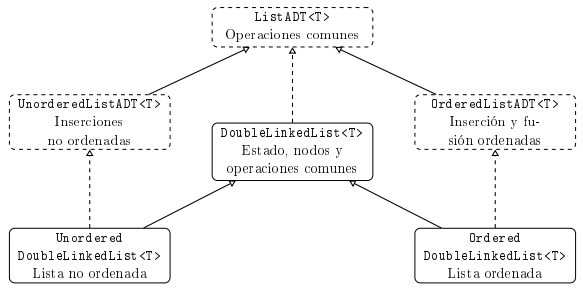
\includegraphics[scale=0.7]{figuras/image.png}
\caption{Diagrama de clases. }

\end{figure}

\chapter{Descripción de las estructuras de datos principales}

Sobre las listas doblemente enlazadas, podemos afirmar que si la lista está vacía, no hay ningún nodo, por lo que \texttt{first == null} y el contador vale cero \texttt{count == 0}. En caso de tener elementos cada nodo desde el primero apuntará tanto al siguiente como al anterior, de manera que el último es accesible desde el primero y el primero desde el último formando un círculo.
En los casos en los que solo hay un nodo, este se apuntará a sí mismo. El contador nos permite saber el número de elementos de manera directa \texttt{O(1)} sin tener que recorrer toda la lista contando elementos, a coste de que cada vez que añadimos o quitamos un elemento de la lista agregar una modificación al contador.
Cada vez que se añade o se retira un elemento de la lista, hay que actualizar los enlaces del elemento nuevo y de los elementos que rodean al nuevo elemento para que no se rompa la lista.

\chapter{Diseño e implementación de los métodos principales}

A continuación se presentan los métodos principales de las listas, con su código y el coste de cada uno. En los costes, $n$ es el número de elementos de la lista y comparar dos elementos cuesta $O(1)$. Los métodos \texttt{isEmpty}, \texttt{size}, \texttt{isAlone}, \texttt{first}, \texttt{last} y \texttt{addWhenEmpty} hacen un número fijo de operaciones $\Rightarrow O(1)$.


\bigskip
\begin{minipage}{0.95\linewidth}
\section{\label{isEmpty}isEmpty}
\begin{lstlisting}[language=Java]
  //comprueba si la lista está vacía.
  public boolean isEmpty() {return first == null;} 
\end{lstlisting}
\end{minipage}\smallskip


\begin{minipage}{0.95\linewidth}
\section{\label{size}size}
\begin{lstlisting}[language=Java]
  //devuelve el número de elementos de la lista.
  public int size() {return count;} 
\end{lstlisting}
\end{minipage}\smallskip


\begin{minipage}{0.95\linewidth}
\section{\label{isAlone}isAlone}
\begin{lstlisting}[language=Java]
  //comprueba si la lista contiene un único nodo.
  public boolean isAlone() {return first == first.next;}
\end{lstlisting}
\end{minipage}\smallskip


\begin{minipage}{0.95\linewidth}
\section{\label{locate}locate}
\begin{lstlisting}[language=Java]
  //busca el nodo cuyo dato es igual a {@code elem}.
  protected Node<T> locate(T elem) {
    if (isEmpty()) {return null;}
    Node<T> aux = first;
    do {
      if (Objects.equals(elem, aux.data)) {return aux;}
      aux = aux.next;
    } while (aux != first);
    return null;
  }
\end{lstlisting}
\end{minipage}\smallskip

\coste{mejor caso (es el primero): 1 comparación $\Rightarrow O(1)$. Peor caso (no está o es el último): $n$ comparaciones de coste constante $\Rightarrow O(n)$.}

\begin{minipage}{0.95\linewidth}
\section{\label{removeFirst}removeFirst}
\begin{lstlisting}[language=Java]
  //Elimina el primer nodo, actualiza {@code first} y los enlaces entre el nuevo primero y el último.
  public T removeFirst() {
    Node<T> aux;
    if (isEmpty()) {
      throw new NoSuchElementException();
    } else {
      aux = first;
      if (isAlone()) {
        first = null;
      } else {
        first.prev.next = first.next;
        first.next.prev = first.prev;
        first = first.next;
      }
      count--;
    }
    return aux.data;
  }
\end{lstlisting}
\end{minipage}\smallskip


\coste{sin recorridos, solo comprobaciones y un número fijo de asignaciones $\Rightarrow O(1)$.}

\begin{minipage}{0.95\linewidth}
\section{\label{removeLast}removeLast}
\begin{lstlisting}[language=Java]
  //Elimina el último nodo y actualiza los enlaces entre el nuevo último y {@code first}.
  public T removeLast() {
    Node<T> aux;
    if (isEmpty()) {
      throw new NoSuchElementException();
    } else {
        aux = first.prev;
        if (isAlone()) {
          first = null;
        } else {
          first.prev.prev.next = first;
          first.prev = first.prev.prev;
        }
        count--;
    }
    return aux.data;
  }
\end{lstlisting}
\end{minipage}\smallskip


\coste{el último es \texttt{first.prev} (lista circular), así que no hay recorrido $\Rightarrow O(1)$. En una lista simple sería $O(n)$.}

\begin{minipage}{0.95\linewidth}
\section{\label{remove}remove}
\texttt{remove} se apoya en \ref{locate} \texttt{locate}
\begin{lstlisting}[language=Java]
  //Busca y elimina el primer elemento igual a {@code elem}, actualizando los enlaces de sus nodos vecinos.
  public T remove(T elem) {
    if (isEmpty()) {throw new NoSuchElementException();}

    Node<T> aux = locate(elem);
    if (aux == null) {return null;}
    if (aux == first) {return removeFirst();}

    aux.prev.next = aux.next;
    aux.next.prev = aux.prev;
    count--;

    return aux.data;
  }
\end{lstlisting}
\end{minipage}\smallskip


\coste{se busca con \texttt{locate} y se enlazan los vecinos: $O(n) + O(1) = O(n)$.}

\begin{minipage}{0.95\linewidth}
\section{\label{first}first}
\begin{lstlisting}[language=Java]
  //Devuelve el primer elemento
  public T first() {
    if (isEmpty()) {
      throw new NoSuchElementException();
    } else {
      return first.data;
    }
  }  
\end{lstlisting}
\end{minipage}\smallskip


\begin{minipage}{0.95\linewidth}
\section{\label{last}last}
\begin{lstlisting}[language=Java]
  //Devuelve el último elemento
  public T last() {
    if (isEmpty()) {
      throw new NoSuchElementException();
    } else {
      return first.prev.data;
    }
  }  
\end{lstlisting}
\end{minipage}\smallskip


\begin{minipage}{0.95\linewidth}
\section{\label{contains}contains}
\texttt{contains} se apoya en \ref{locate} \texttt{locate}
\begin{lstlisting}[language=Java]
  //Comprueba si la lista contiene un elemento igual a {@code elem}
  public boolean contains(T elem) {
    Node<T> aux;
    if (isEmpty()) {
      return false;
    } else {
      aux = locate(elem);
      if (aux != null) {
        return Objects.equals(aux.data, elem);
      } else {
        return false;
      }
    }
  }
\end{lstlisting}
\end{minipage}\smallskip


\coste{solo llama a \texttt{locate} $\Rightarrow O(n)$.}

\begin{minipage}{0.95\linewidth}
\section{\label{find}find}
\texttt{find} se apoya en \ref{locate} \texttt{locate}
\begin{lstlisting}[language=Java]
    public T find(T elem) {
        Node<T> aux;
        if (isEmpty()) {
            return null;
        } else {
            aux = locate(elem);
            if (aux == null) {
                return null;
            }
            if (Objects.equals(aux.data, elem)) {
                return aux.data;
            } else {
                return null;
            }
        }
    }
\end{lstlisting}
\end{minipage}\smallskip

\coste{igual que \texttt{contains}, solo depende de \texttt{locate} $\Rightarrow O(n)$.}

\begin{minipage}{0.95\linewidth}
\section{\label{addWhenEmpty}addWhenEmpty}
\begin{lstlisting}[language=Java]
  //Crea el único nodo de la lista vacía y enlaza sus referencias {@code next} y {@code prev} consigo mismo.
  public void addWhenEmpty(T elem) {
    Node<T> newNode = new Node<>(elem);
    newNode.next = newNode;
    newNode.prev = newNode;
    first = newNode;
    count++;
  }
\end{lstlisting}
\end{minipage}\smallskip

\begin{minipage}{0.95\linewidth}
\section{\label{insertAdd}insertAdd}
\texttt{insertAdd} inserta entre dos nodos que ya recibe, por lo que no recorre la lista.
\begin{lstlisting}[language=Java]
  //Inserta {@code elem} entre los nodos {@code prev} y {@code next}, actualizando {@code prev.next} y {@code next.prev}.
  public void insertAdd(T elem, Node<T> prev, Node<T> next) {
    Node<T> newNode = new Node<>(elem, prev, next);
    prev.next = newNode;
    next.prev = newNode;
    count++;
  }
\end{lstlisting}
\end{minipage}\smallskip

\coste{crear el nodo y actualizar \texttt{prev.next}, \texttt{next.prev} y \texttt{count} $\Rightarrow O(1)$.}

\begin{minipage}{0.95\linewidth}
\section{\label{actualizarFirst}actualizarFirst}
\begin{lstlisting}[language=Java]
  //Cambia la referencia al primer nodo; no modifica los enlaces ni el número de elementos.
  public void actualizarFirst(Node<T> node) {first = node;}
\end{lstlisting}
\end{minipage}\smallskip

\coste{una sola asignación $\Rightarrow O(1)$.}

\begin{minipage}{0.95\linewidth}
\section{\label{insertFirst}insertFirst}
\begin{lstlisting}[language=Java]
  //Inserta {@code elem} al principio y actualiza {@code first}
  public void insertFirst(T elem) {
    if (isEmpty()) {
      addWhenEmpty(elem);
      return;
    }
    insertAdd(elem, first.prev, first);
    first = first.prev;
  }
\end{lstlisting}
\end{minipage}\smallskip

\coste{\texttt{insertAdd} y mover \texttt{first}: $O(1) + O(1) = O(1)$.}

\begin{minipage}{0.95\linewidth}
\section{\label{iterator}iterator}
\begin{lstlisting}[language=Java]
  public Iterator<T> iterator() {return new ListIterator();}
  private class ListIterator implements Iterator<T> {
    private Node<T> aux = first;
    private int contador = count;
    @Override
    public boolean hasNext() {return contador > 0;}
    @Override
    public T next() {
      if (!hasNext()) {throw new NoSuchElementException();}
      T data = aux.data;
      aux = aux.next;
      contador--;
      return data;
    }
  }
\end{lstlisting}
\end{minipage}\smallskip


\coste{\texttt{hasNext} y \texttt{next} cuestan $O(1)$. Recorrer toda la lista: $n \cdot O(1) = O(n)$.}

\begin{minipage}{0.95\linewidth}
\section{\label{toString}toString}
\begin{lstlisting}[language=Java]
  //Concatena la representación de todos los elementos.
  public String toString() {
    String result = new String();
    Iterator<T> it = iterator();
    while (it.hasNext()) {
      T elem = it.next();
      result = result + "[" + elem.toString() + "] \n";
    }
    return "DoubleLinkedList " + result + "]";
  }
\end{lstlisting}
\end{minipage}\smallskip

\coste{el recorrido es $O(n)$, pero cada concatenación copia todo lo acumulado:
\[ \sum_{i=1}^{n} i = \frac{n(n+1)}{2} \;\Rightarrow\; O(n^2) \]}

\begin{table}[ht]
\section{\label{tablaResumen}Resumen de costes comunes}
\begin{minipage}{0.95\linewidth}
\centering
\renewcommand{\arraystretch}{1.3}
\begin{tabular}{>{\ttfamily}l l}
\toprule
\normalfont Operación & complejidad\\
\midrule
isEmpty & $O(1)$\\
size & $O(1)$\\
isAlone & $O(1)$\\
locate & $O(n)$\\
removeFirst & $O(1)$\\
removeLast & $O(1)$\\
remove & $O(n)$\\
first & $O(1)$\\
last & $O(1)$\\
contains & $O(n)$\\
find & $O(n)$\\
addWhenEmpty & $O(1)$\\
insertAdd & $O(1)$\\
actualizarFirst & $O(1)$\\
insertFirst & $O(1)$\\
iterator & $O(1)$\\
toString & $O(n^2)$\\

\bottomrule
\end{tabular}
\caption{Costes de las operaciones comunes.}
\end{minipage}\smallskip
\end{table}

\begin{minipage}{0.95\linewidth}
\section{\label{addTo}addTo}
\begin{lstlisting}[language=Java]
  //Inserta un elemento al principio o al final
  private void addTo(T elem, boolean front) {
    if (isEmpty()) {
      addWhenEmpty(elem);
    } else {
      insertAdd(elem, first.prev, first);
      if (front) {actualizarFirst(first.prev);}
    }
  }
\end{lstlisting}
\end{minipage}\smallskip

\coste{\texttt{insertAdd} (y \texttt{actualizarFirst} si es al principio) $\Rightarrow O(1)$.}

\begin{minipage}{0.95\linewidth}
\section{\label{UnorderedfindOrAdd}UnorderedfindOrAdd}
\begin{lstlisting}[language=Java]
  //Busca un elemento igual a {@code elem} o lo inserta en orden. {@code n} es el tamaño de la lista.
  public T findOrAdd(T elem) {
    if (isEmpty()) {
      addWhenEmpty(elem);
      return elem;
    }
    Node<T> aux = locate(elem);
    if (aux == null) {addToRear(elem);}
    return elem;
  }
 
\end{lstlisting}
\end{minipage}\smallskip

\coste{\texttt{locate} y después \texttt{addToRear}: $O(n) + O(1) = O(n)$. Mejor caso (vacía o es el primero): $O(1)$.}

\begin{minipage}{0.95\linewidth}
\section{\label{addToFront}addToFront}
\begin{lstlisting}[language=Java]
  //Inserta {@code elem} entre el primero y el ultimo y actualiza {@code first} y los enlaces entre el nuevo nodo y los extremos de la lista.
  public void addToFront(T elem) {
    addTo(elem, true);
  }
 
\end{lstlisting}
\end{minipage}\smallskip

\begin{minipage}{0.95\linewidth}
\section{\label{addToRear}addToRear}
\begin{lstlisting}[language=Java]
  //Inserta {@code elem} entre el primero y el ultimo y actualiza los enlaces entre el nuevo nodo y los extremos de la lista.
  public void addToRear(T elem) {
    addTo(elem, false);
  }
 
\end{lstlisting}
\end{minipage}\smallskip

\coste{\texttt{addToFront} y \texttt{addToRear} solo llaman a \texttt{addTo} $\Rightarrow O(1)$.}

\begin{minipage}{0.95\linewidth}
\section{\label{addAfter}addAfter}
\begin{lstlisting}[language=Java]
  //Busca {@code target} e inserta {@code elem} a continuación, actualizando los enlaces de los nodos vecinos. 
  //Si la lista está vacía, inserta primero {@code target} y después {@code elem}.
  //Si no está vacía y no encuentra {@code target}, no modifica la lista.
  public void addAfter(T elem, T target) {
    if (isEmpty()) {
      addWhenEmpty(target);
      addAfter(elem, target);
    } else {
      Node<T> nodoTarget = locate(target);
      if (nodoTarget != null) {insertAdd(elem, nodoTarget, nodoTarget.next);}
    }
  }
 
\end{lstlisting}
\end{minipage}\smallskip

\coste{lista no vacía: \texttt{locate} y \texttt{insertAdd}, $O(n) + O(1) = O(n)$. Lista vacía: se inserta \texttt{target} y se encuentra a la primera $\Rightarrow O(1)$.}

\begin{table}[ht]
\section{\label{tablaResumenUnordered}Resumen de costes de la lista no ordenada}
\begin{minipage}{0.95\linewidth}
\centering
\renewcommand{\arraystretch}{1.3}
\begin{tabular}{>{\ttfamily}l l}
\toprule
\normalfont Operación & complejidad\\
\midrule
addTo & $O(1)$\\
findOrAdd & $O(n)$\\
addToFront & $O(1)$\\
addToRear & $O(1)$\\
addAfter & $O(n)$\\


\bottomrule
\end{tabular}
\caption{Costes de las operaciones de la lista no ordenada.}
\end{minipage}\smallskip
\end{table}

\begin{minipage}{0.95\linewidth}
\section{\label{add}add}
\begin{lstlisting}[language=Java]
  //Inserta {@code elem} en orden si no existe. {@code n} es el tamaño de la lista.
  public void add(T elem) {
    if (isEmpty()) {
      addWhenEmpty(elem);
      return;
    }
    Node<T> last = first.prev;
    if (elem.compareTo(first.data) == 0 || elem.compareTo(last.data) == 0) {return;}
    if (elem.compareTo(last.data) > 0) {
      insertAdd(elem, last, first);
      return;
    }
    if (elem.compareTo(first.data) < 0) {
      insertAdd(elem, last, first);
      actualizarFirst(first.prev);
      return;
    }
    Node<T> current = first;
    while (current.next != first && elem.compareTo(current.next.data) > 0) {current = current.next;}
    if (elem.compareTo(current.next.data) == 0) {return;}
    insertAdd(elem, current, current.next);
  }
\end{lstlisting}
\end{minipage}\smallskip

\coste{mejor caso: se compara solo con \texttt{first} y \texttt{last} $\Rightarrow O(1)$. Peor caso: el elemento queda entre medias y se recorren hasta $n$ nodos $\Rightarrow O(n)$.}

\begin{minipage}{0.95\linewidth}
\section{\label{OrderedfindOrAdd}OrderedfindOrAdd}
\begin{lstlisting}[language=Java]
  //Busca un elemento igual a {@code elem} o lo inserta en orden. {@code n} es el tamaño de la lista.
  public T findOrAdd(T elem) {
    if (isEmpty()) {
      addWhenEmpty(elem);
      return elem;
    }
    int comparacionConPrimero = elem.compareTo(first.data);
    if (comparacionConPrimero == 0) {return first.data;}
    if (comparacionConPrimero < 0) {
      insertAdd(elem, first.prev, first);
      actualizarFirst(first.prev);
      return elem;
    }
    Node<T> last = first.prev;
    int comparacionConUltimo = elem.compareTo(last.data);
    if (comparacionConUltimo == 0) {return last.data;}
    if (comparacionConUltimo > 0) {
      insertAdd(elem, last, first);
      return elem;
    }
    Node<T> current = first;
    while (elem.compareTo(current.next.data) > 0) {current = current.next;}
    int comparacionConSiguiente = elem.compareTo(current.next.data);
    if (comparacionConSiguiente == 0) {return current.next.data;}
    insertAdd(elem, current, current.next);
    return elem;
  }
\end{lstlisting}
\end{minipage}\smallskip

\coste{igual que \texttt{add}: mejor caso $O(1)$, peor caso $O(n)$.}

\begin{minipage}{0.95\linewidth}
\section{\label{merge}merge}
\begin{lstlisting}[language=Java]
  //En recorridos e inserciones: fusiona ambas listas en orden. {@code n} y {@code m} son sus tamaños iniciales; combinar elementos iguales añade el coste de {@code combinarCon}.
  public void merge(DoubleLinkedList<T> lista) {
    if (lista == null || lista.first == null) {return;}
    if (isEmpty()) { // si nuestra lista esta vacia se clona con la del parametro
      first = lista.first;
      count = lista.count;
      return;
    }
    Node<T> p1 = first; // creamos los punteros para que recorran las listas
    Node<T> p2 = lista.first;
    int cuantos1 = count; // guardamos en auxiliares la cantidad total de elementos de cada lista.
    int cuantos2 = lista.count;
    while (cuantos1 > 0 && cuantos2 > 0) { // fusionamos ambas listas
      if (p1.data.compareTo(p2.data) < 0) { // si esta ordenado, seguimos comprobando
        p1 = p1.next;
        cuantos1--;
      } else if (p1.data.compareTo(p2.data) == 0) {
        combinarIguales(p1.data, p2.data);
        p1 = p1.next;
        p2 = p2.next;
        cuantos1--;
        cuantos2--;
      } else { // si no reemplazamos
        insertAdd(p2.data, p1.prev, p1); // si esta desordenado, añadimos en nuestra lista el elemento anterior a p1.
        if (p1 == first) { // comprobamos si hemos añadido un elemento antes del first
          actualizarFirst(first.prev); // p2 pasa a ser el nuevo first de nuestra lista
        }
        p2 = p2.next; // actualizamos el puntero de la lista del segundo 
        cuantos2--;
      }
    }
    // si aun quedan elementos en la otra lista, entonces es que quedan los mayores, por lo que irian al final.
    while (cuantos2 > 0) {
      insertAdd(p2.data, first.prev, first); // insertamos cada elemento al final en orden
      p2 = p2.next;
      cuantos2--;
    }
  }
\end{lstlisting}
\end{minipage}\smallskip

\coste{$n$ y $m$ son los tamaños de las dos listas. Si alguna está vacía, $O(1)$ (con la actual vacía solo se copian \texttt{first} y \texttt{count}). En el caso general cada vuelta del bucle avanza en al menos una lista y cuesta $O(1)$:
\[ \mbox{vueltas} \leq n + m \;\Rightarrow\; O(n + m) \]
Cada pareja de elementos iguales suma una llamada a \texttt{combinarIguales}.}

\begin{minipage}{0.95\linewidth}
\section{\label{combinarIguales}combinarIguales}
\begin{lstlisting}[language=Java]
  //Combina las X de {@code otro} con las de este Y. {@code n} es el número de X de {@code otro}, {@code m} el número inicial de X de este Y y {@code k} el máximo de Y asociados a una X.
  //Siendo X Actor o Pelicula e Y el que no sea X
  private void combinarIguales(T actual, T entrante) {
    if (actual instanceof Actor actor) {
      actor.combinarCon((Actor) entrante);
    } else if (actual instanceof Pelicula pelicula) {
      pelicula.combinarCon((Pelicula) entrante);
    }
  }
\end{lstlisting}
\end{minipage}\smallskip

\coste{solo llama a \texttt{combinarCon} (de \texttt{Actor} o de \texttt{Pelicula}), así que cuesta lo mismo que ese método. Para dos actores, $n$ son las películas del actor que entra, $m$ las que ya tenía el nuestro y $k$ el máximo de actores de una película (no son las letras de \texttt{merge}). Por cada una de las $n$ películas hay dos \texttt{findOrAdd}, uno en las películas del actor ($\leq m + n$ elementos) y otro en los actores de la película ($\leq k$):
\[ n \cdot \bigl( O(m + n) + O(k) \bigr) = O\bigl(n(m + n + k)\bigr) \]
Con dos películas es igual, intercambiando los papeles.}

\begin{table}[ht]
\section{\label{tablaResumenOrdered}Resumen de costes de la lista ordenada}
\begin{minipage}{0.95\linewidth}
\centering
\renewcommand{\arraystretch}{1.3}
\begin{tabular}{>{\ttfamily}l p{8cm}}
\toprule
\normalfont Operación & complejidad\\
\midrule
add & $O(n)$\\
OrderedfindOrAdd & $O(n)$\\
merge & $O(n + m)$ + llamadas a \texttt{combinarIguales}\\
combinarIguales & $O(n(m + n + k))$\\


\bottomrule
\end{tabular}
\caption{Costes de las operaciones de la lista ordenada.}
\end{minipage}\smallskip
\end{table}

\section{Pruebas realizadas}
Se han implementado 18 pruebas con JUnit 5, agrupadas por clase.

\subsection*{Lista ordenada (\texttt{OrderedDoubleLinkedListTest})}
\begin{itemize}
\item \texttt{testOrdenYDuplicados}: inserta C, A, B y un A repetido; comprueba que quedan 3 elementos en orden A, B, C.
\item \texttt{testFindOrAdd}: \texttt{findOrAdd} con un elemento nuevo y con uno repetido; el tamaño no crece con el repetido.
\item \texttt{testMergeVaciaConVacia}: fusionar dos listas vacías deja la lista vacía.
\item \texttt{testMergeVaciaConDatos}: fusionar una lista con datos en una lista vacía.
\item \texttt{testMergeConDatosConVacia}: fusionar una lista vacía en una con datos no la modifica.
\item \texttt{testMergeRangosSeparados}: listas con rangos que no se solapan (A, B con C, D).
\item \texttt{testMergeRangosIntercalados}: listas con elementos intercalados (A, C con B, D); el resultado queda ordenado.
\item \texttt{testMergeConIDsRepetidos}: dos \texttt{Actor} con el mismo identificador se combinan en uno que conserva los dos años.
\item \texttt{testAutoFusion}: fusionar una lista consigo misma no lanza excepción.
\end{itemize}

\subsection*{Lista no ordenada (\texttt{UnorderedDoubleLinkedListTest})}
\begin{itemize}
\item \texttt{testAddAfterSinTarget}: \texttt{addAfter} con un objetivo ausente en una lista no vacía no modifica la lista.
\item \texttt{testAddToRearaddAfter}: con películas, \texttt{addToRear} y \texttt{addAfter} dejan los elementos en el orden esperado.
\item \texttt{testInsertarFrontRear}: \texttt{addToFront} y \texttt{addToRear} en lista vacía, de un elemento y de varios; se comprueban \texttt{first}, \texttt{last} y \texttt{size}.
\item \texttt{testAddAfterListaVacia}: \texttt{addAfter} en lista vacía, con objetivo presente y con objetivo ausente.
\item \texttt{testContainsYFind}: \texttt{contains} y \texttt{find} en lista vacía, con elemento presente y con elemento ausente.
\item \texttt{testEliminaciones}: excepciones en lista vacía; eliminación de un elemento intermedio, del primero, del último y del único restante.
\end{itemize}

\subsection*{Integración con la práctica 1 (\texttt{LectorPeliculasActoresTest})}
\begin{itemize}
\item \texttt{leeActoresYPeliculasDelFichero}: cantidades de registros, actores y películas, algunos actores concretos y búsqueda por identificador.
\item \texttt{testRelacionesActorPeliculaConLotes}: las relaciones entre actores y películas existen en ambos sentidos y no se repiten identificadores.
\item \texttt{noDuplicaRelacionesActorPeliculaRepetidas}: las 11 filas de \textit{Super López} corresponden a 10 actores únicos, porque Dani Rovira aparece en 2015 y 2018.
\end{itemize}

\chapter{Código}
Para una mejor lectura del código, se facilita el enlace al GitHub público:
\begin{itemize}
\item \url{https://github.com/erasmosee/EDA_Practica2_LinkedList}
\end{itemize}

\chapter{Conclusiones}
La práctica nos ha servido para ver el potencial que tienen las listas enlazadas cuando cumplen los criterios de estar doblemente enlazadas y de ser una lista circular, frente a listas enlazadas más simples, si bien es cierto que la memoria usada por las listas doblemente enlazadas es bastante superior a las listas enlazadas de una sola dirección, consideramos que es un coste asumible a la hora de proceder a trabajar con dichas listas.

\section{\label{dificultades}Dificultades}

Durante el desarrollo de la práctica 2, hemos ido probando distintas formas de integrarla con la práctica 1, pues era un objetivo que ya teníamos en mente desde el principio.

En un primer momento antes de implementar el método \texttt{merge}, procedíamos a volcar la información leída de los ficheros a un hashmap, ordenarlo y posteriormente lo volcábamos a una \texttt{OrderedDoubleLinkedList}, como es de suponer, la velocidad de insertar elementos ordenados en una lista ordenada es O(1) siempre que compares previamente el elemento a insertar con el first y con el prev.

Más tarde, tuvimos un método merge no cuadrático, y fue cuando empezamos a tener pequeñas listas sacadas una de cada fichero de año, las cuales obteníamos aun mediante hashmap, pero que las volcábamos a OrderedDoubleLinkedList para luego proceder a mergearlas en una única lista OrderedDoubleLinkedList, en este momento fue cuando el programa pasó de tardar de 12 minutos a 70 segundos en procesar la lista completa de actores y películas.

Una vez llegados a este punto en el que el programa tardaba \textquotedblleft solo\textquotedblright{} 70 segundos, y lo comentábamos contentos pues sabíamos de donde veníamos, empezamos una pequeña competición por hacer un merge decente.

Mientras unos estaban con el merge, otros estaban dilucidando como reducir esos 70 segundos con los que en ese momento estábamos contentos, por lo que empezamos a pensar en hacer merge de listas más pequeñas a medida que leíamos de cada fichero.

En un principio pensamos que cada 1000 elementos podíamos hacer un merge por lo que modificamos el lector para que cuando llevase X elementos mergease lo leído a una \texttt{OrderedDoubleLinkedList} de los datos de ese año, para una vez finalizado el fichero de año, mergearlo con la \texttt{OrderedDoubleLinkedList} global.

Ya que teníamos un número, decidimos empezar a variarlo y comprobar como respondía el código, para nuestra sorpresa, el número bueno no era mil elementos, sino 128, y es en ese punto donde descubrimos que se realizaban el menor número de operaciones \texttt{compareTo} en nuestro código.

Ni que decir que cuanto más aproximábamos el número de lotes a 128 más rápido se procesaba el código, las últimas pruebas ya fueron para ajustar milésimas, es cuando habíamos llegado a menos de 3 segundos.


\begin{table}[ht]
\section{\label{tablaTiemposComparacionesMerge}Tiempos y comparaciones del merge elegido}
\begin{minipage}{0.95\linewidth}
  Dado que mergePruebas realizaba siempre más operaciones se optó por descartarlo y usar mergeEficaz, el cual fue renombrado a merge.

\centering
\begin{tabular}{>{\ttfamily}l l l l l}
\toprule
\normalfont Tipo de lectura & Tipo de Merge & Tamaño lote & Tiempo (ms) & Comparaciones \\
\midrule
LinkedList & eficaz & 0100 & 3008 & 84505092\\
LinkedList & eficaz & 0101 & 2972 & 84382285\\
LinkedList & eficaz & 0102 & 2990 & 84233346\\
LinkedList & eficaz & 0103 & 3005 & 84050349\\
LinkedList & eficaz & 0104 & 2960 & 83982697\\
LinkedList & eficaz & 0105 & 2993 & 83796540\\
LinkedList & eficaz & 0106 & 2998 & 83708411\\
LinkedList & eficaz & 0107 & 2958 & 83577457\\
LinkedList & eficaz & 0108 & 3004 & 83476276\\
LinkedList & eficaz & 0109 & 2907 & 83377290\\
LinkedList & eficaz & 0110 & 3019 & 83296420\\
LinkedList & eficaz & 0111 & 3028 & 83179341\\
LinkedList & eficaz & 0112 & 3014 & 83155664\\
LinkedList & eficaz & 0113 & 3033 & 83048387\\
LinkedList & eficaz & 0114 & 2918 & 82956969\\
LinkedList & eficaz & 0115 & 3001 & 82927237\\
LinkedList & eficaz & 0116 & 2975 & 82840151\\
LinkedList & eficaz & 0117 & 3174 & 82862973\\
LinkedList & eficaz & 0118 & 3061 & 82731382\\
LinkedList & eficaz & 0119 & 2852 & 82737519\\
LinkedList & eficaz & 0120 & 2878 & 82697094\\
LinkedList & eficaz & 0121 & 2975 & 82718085\\
LinkedList & eficaz & 0122 & 2890 & 82650588\\
LinkedList & eficaz & 0123 & 2966 & 82635178\\
LinkedList & eficaz & 0124 & 2977 & 82638738\\
LinkedList & eficaz & 0125 & 2918 & 82654824\\
LinkedList & eficaz & 0126 & 2994 & 82634253\\
LinkedList & eficaz & 0127 & 2940 & 82600991\\
LinkedList & eficaz & 0128 & 2900 & 82594718\\
LinkedList & eficaz & 0129 & 2972 & 82656716\\
LinkedList & eficaz & 0130 & 2968 & 82667334\\
LinkedList & eficaz & 0131 & 3009 & 82604169\\
LinkedList & eficaz & 0132 & 3019 & 82652078\\
LinkedList & eficaz & 0133 & 2939 & 82702540\\
LinkedList & eficaz & 0134 & 3000 & 82766518\\
LinkedList & eficaz & 0135 & 2943 & 82778629\\
LinkedList & eficaz & 0136 & 2950 & 82816234\\
LinkedList & eficaz & 0137 & 2939 & 82837771\\
LinkedList & eficaz & 0138 & 2874 & 82834454\\
LinkedList & eficaz & 0139 & 2910 & 82945814\\
LinkedList & eficaz & 0140 & 2925 & 82985020\\

\bottomrule
\end{tabular}
\caption{Número de operaciones por tamaños de lotes y tiempo de operación en (ms) del merge elegido.}
\end{minipage}\smallskip
\end{table}


\begin{table}[ht]
\section{\label{tablaTiemposComparacionesOtrosMerge}Tiempos y comparaciones de otros merges}
\begin{minipage}{0.95\linewidth}
  Dado que mergePruebas realizaba siempre más operaciones se optó por descartarlo y usar mergeEficaz, el cual fue renombrado a merge.

\centering
\begin{tabular}{>{\ttfamily}l l l l l}
\toprule
\normalfont Tipo de lectura & Tipo de Merge & Tamaño lote & Tiempo (ms) & Comparaciones \\
\midrule
HashMap & eficaz & 0000 & 4211 & 30.948.898\\
HashMap & eficaz & 0000 & 4249 & 30.948.898\\
HashMap & eficaz & 0000 & 4268 & 30.948.898\\
HashMap & eficaz & 0000 & 4275 & 30.948.898\\
\midrule
HashMap & pruebas & 0000 & 4121 & 42.431.698\\
HashMap & pruebas & 0000 & 4186 & 42.431.698\\
\midrule
LinkedList & pruebas & 0000 & 75663 & 2.359.061.629\\
LinkedList & pruebas & 0000 & 78484 & 2.359.061.629\\
LinkedList & pruebas & 0100 & 6804 & 198.922.278\\
LinkedList & pruebas & 0250 & 5600 & 160.686.346\\
LinkedList & pruebas & 0500 & 6148 & 199.115.873\\
LinkedList & pruebas & 1000 & 8053 & 304.985.577\\
LinkedList & pruebas & 2000 & 12932 & 505.847.776\\
\bottomrule
\end{tabular}
\caption{Número de operaciones por tamaños de lotes y tiempo de operación en (ms) de otros merges.}
\end{minipage}\smallskip
\end{table}

\end{document}